\documentclass[a4paper]{article}

\usepackage[utf8]{inputenc}

\usepackage{url}
\usepackage[hidelinks]{hyperref}

\usepackage{caption}

\usepackage{listings}

\usepackage{color}

\usepackage{enumitem}

% *** GRAPHICS RELATED PACKAGES ***
%\usepackage[pdftex]{graphicx}
\usepackage{graphicx}
%\usepackage[dvips]{graphicx}
% to place figures on a fixed position
\usepackage{float}

\usepackage[margin=1in]{geometry}

\title{IoT Lab}
\author{}
\date{}


\begin{document}

\maketitle

\tableofcontents

\section{IoT lab measurement exercises}

In the first phase of the lab a micro-controller will be transformed into a mote. A sensor mote is capable of detect various parameters of its environment and is capable of communication. For this purpose a sensor and a radio module is going to be attached to the micro-controller. For this same device an actuator is going to be connected to it. Furthermore a simple display device is also connected to the already built hierarchy.

In the second phase of the lab a virtual device is created using one of the cloud IoT provider's services that is going to accept and process the data arriving from our physical sensor. The service is going to store and display the data. Furthermore a virtual controller is attached to the virtual sensor that is going to send control signals for the physical device. A gateway device is used for translating the data into the right format between the physical and virtual devices.

The arrangement of these components can be seen on Figure~\ref{fig:meas-arrangement}. The task of the students attending this lab is to program the devices and the gateway for the achieving the desired operation.

\begin{figure}[H]
    \centering
    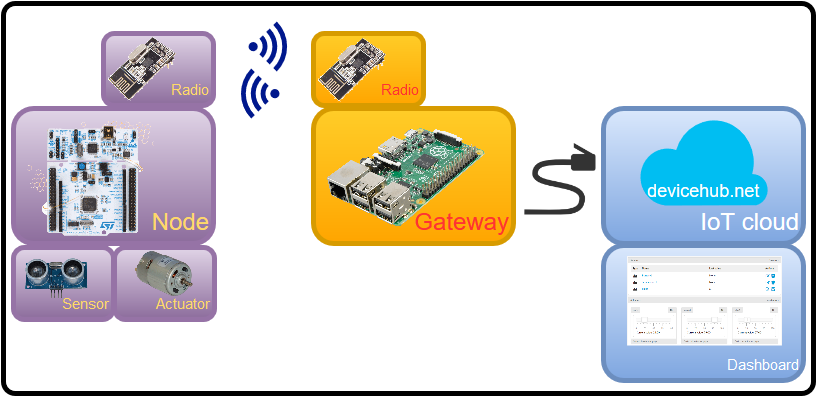
\includegraphics[width=0.9\textwidth]{figures/devices-arrangement.png}
    \caption{Arrangement of devices and components used in this lab}
    \label{fig:meas-arrangement}
\end{figure}

During the exercises a lab report has to be created. In this report the students must document the actions carried out, the code written, the configuration files created etc. The lab report can also contain screen captures. The basic guideline is to create such a document of which the measurement is easily reproducible. 

\section{Getting started with \emph{\textbf{mbed}} environment}

mbed is an IDE (and also an operating system) tailored for IoT applications based 32 bit ARM micro-controllers. There are several commercially available boards available as a result it allows simple and rapid prototyping. One of its main advantages compared to other IDEs that it can handle multiple types of micro-controllers so that the code written can be reused in multiple environments. Furthermore its UI is intuitive and also supports on-line workflows with team integration and version control. Naturally there are some cons as well namely that from mbed the low-level hardware components are not reachable from it and sometimes the basis of the framework called \emph{mbed OS} might contain bugs.

The micro-controller used during this lab is of type NUCLEO-F446RE.

\subsection{First steps}

Before proceeding any further register on site \url{https://developer.mbed.org/}. The registration is simple and easy and doesn't require instant verification of our e-mail addresses. After successful registration log-in on the website and then
\begin{enumerate}
  \item Go to ``Platforms" tab where the development board is selected
  \item Filter the results for manufacturer of "STMicroelectronics"
\end{enumerate}
\begin{figure}[H]
    \centering
    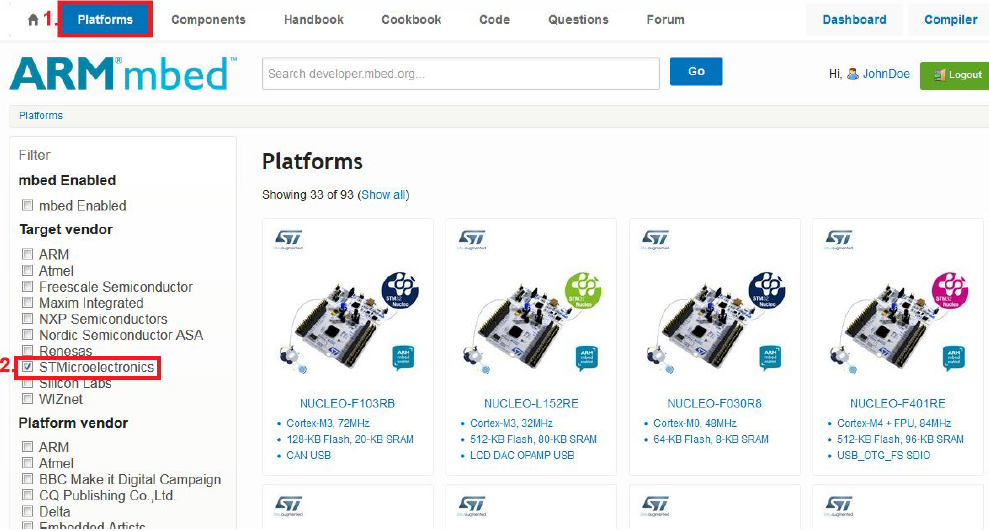
\includegraphics[width=0.9\textwidth]{figures/mbed-platform.png}
\end{figure}
\begin{enumerate}[resume]
\item Search for and select ``NUCLEO-F446RE" dev board. Here we can find detailed description on the micro-controller and also the schematics for the pin to feature connector assignment and functions associated with them
\end{enumerate}
\begin{figure}[H]
    \centering
    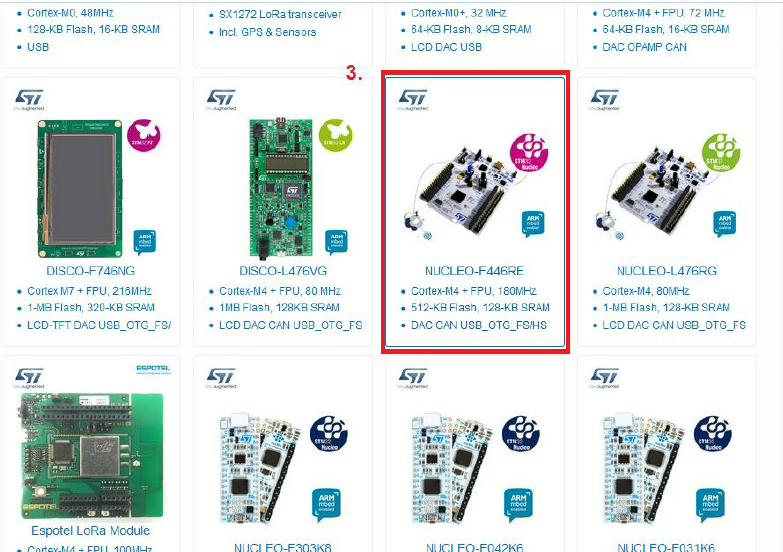
\includegraphics[width=0.9\textwidth]{figures/mbed-nucleo.png}
\end{figure}
\begin{enumerate}[resume]
\item Add the selected board to the compiler by clicking on the ``Add to your mbed Compiler" and the open it using the link in the upper right corner (5.)
\end{enumerate}
\begin{figure}[H]
    \centering
    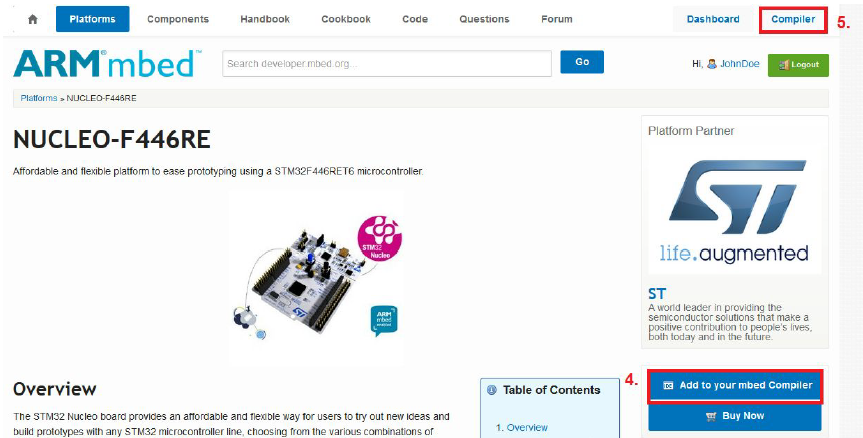
\includegraphics[width=0.9\textwidth]{figures/mbed-compiler.png}
\end{figure}

\subsection{Sample programs and binary upload to the device}

Click on ``New" in the top left corner (1.). In the pop-up window (2.) select the appropriate device type, and then we can select from one of the existing sample projects (or alternatively create a new one) and give a name for it. With the tick-box in the bottom we can select whether to update our code if one of the dependent libraries are updated. Click on OK and afterwards the newly created program will be visible under the My Programs section with the chosen name.
\begin{figure}[H]
    \centering
    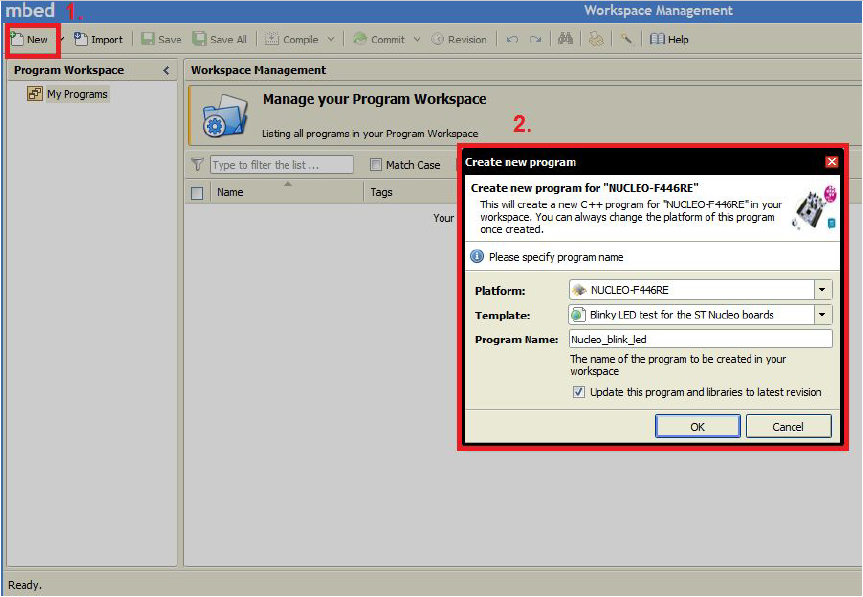
\includegraphics[width=0.9\textwidth]{figures/mbed-new.png}
\end{figure}

We can open and edit (1.) the source file by clicking on it in the left pane. As soon as we are done with the modifications the compilation can be started by clicking on ``Compile" button (2.). If there were no errors and the program compiles successfully the result will be file download pop-up for the resulting binary (3.)

\begin{figure}[H]
    \centering
    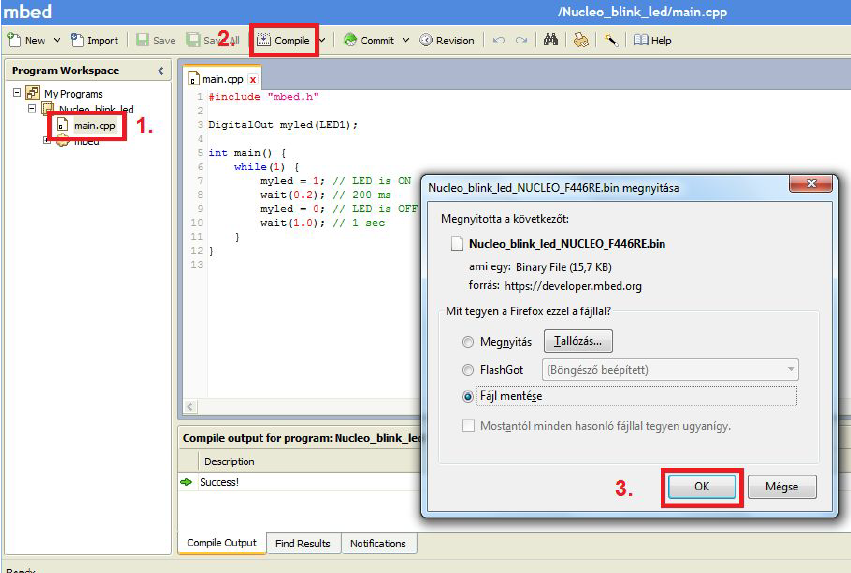
\includegraphics[width=0.9\textwidth]{figures/mbed-compile.png}
\end{figure}

Download/save this binary on the volume created by the dev board (NUCLEO). The green LED will start blinking during software upload to the micro-controller. If there are no errors our code will run on the device.

\begin{figure}[H]
    \centering
    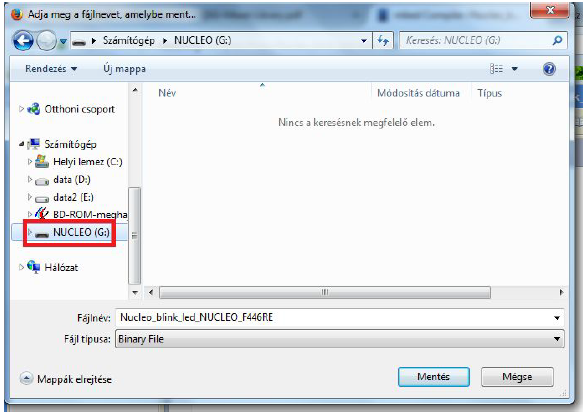
\includegraphics[width=0.9\textwidth]{figures/mbed-nucleo-save.png}
\end{figure}

\subsection{Creating an empty project}
Similarly to the previous steps click on ``New" (1.) then select "Empty Program" option (2.). Name the project (3.) then click OK. (4.)

\begin{figure}[H]
    \centering
    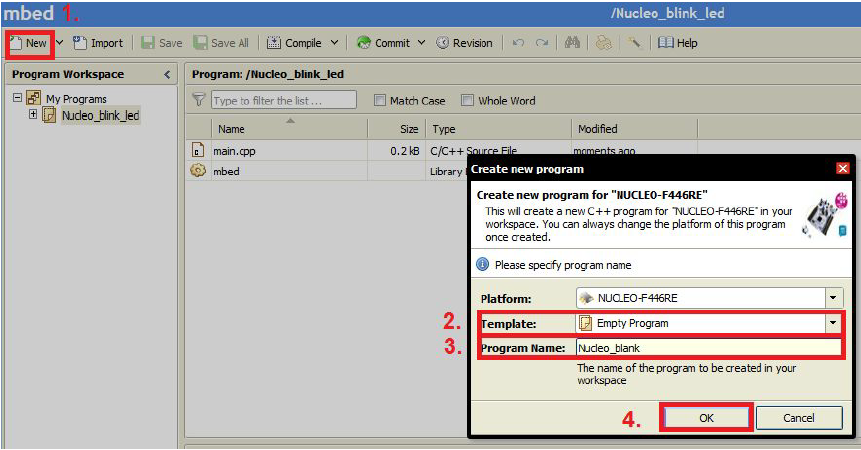
\includegraphics[width=0.9\textwidth]{figures/mbed-empty-proj.png}
\end{figure}

The empty application project needs at least the mbed runtime library that can be added to the project in the following way:
\begin{enumerate}
  \setcounter{enumi}{0}
  \item Select the project
  \item click on ``Import"
  \item select the ``Libraries" tab
  \item search for the word ``mbed"
  \item Import
\end{enumerate}

\begin{figure}[H]
    \centering
    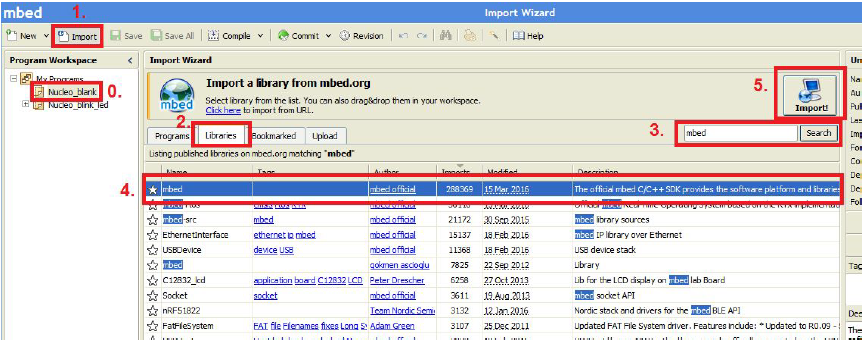
\includegraphics[width=0.9\textwidth]{figures/mbed-import.png}
\end{figure}

\subsection{Different ways of importing}

There are some other ways for importing programs and libraries. A program can be imported based on the above describe method but selecting the ``Programs" tab (1.).
A program or library can be either uploaded from our local machine from a file (2.) or we can download it given that the url of it is know and we have sufficient privileges.

\begin{figure}[H]
    \centering
    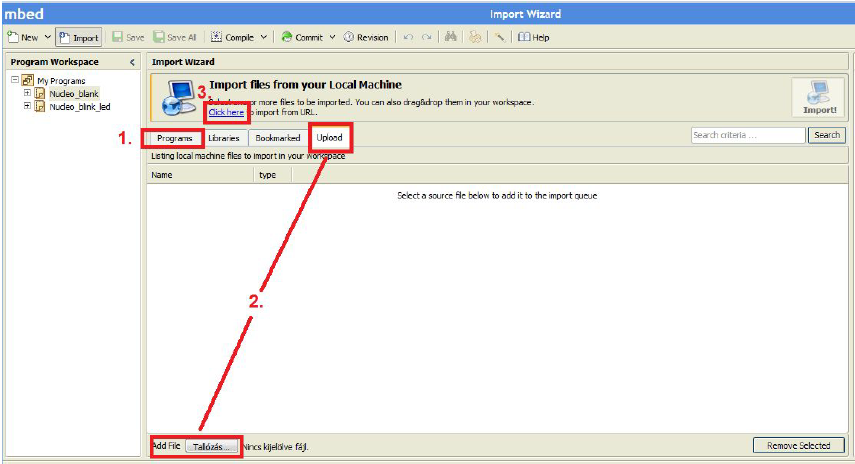
\includegraphics[width=0.9\textwidth]{figures/mbed-import2.png}
\end{figure}

In case if we are a part of a development team there is an option for importing the sources published by other developers.

\begin{figure}[H]
    \centering
    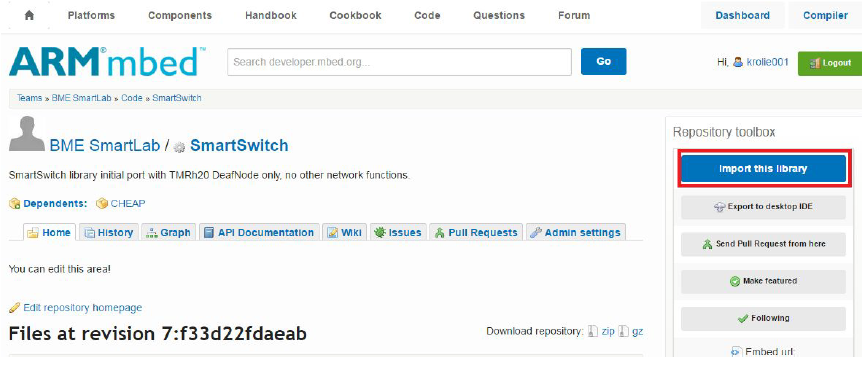
\includegraphics[width=0.9\textwidth]{figures/mbed-online-import.png}
\end{figure}
\begin{figure}[H]
    \centering
    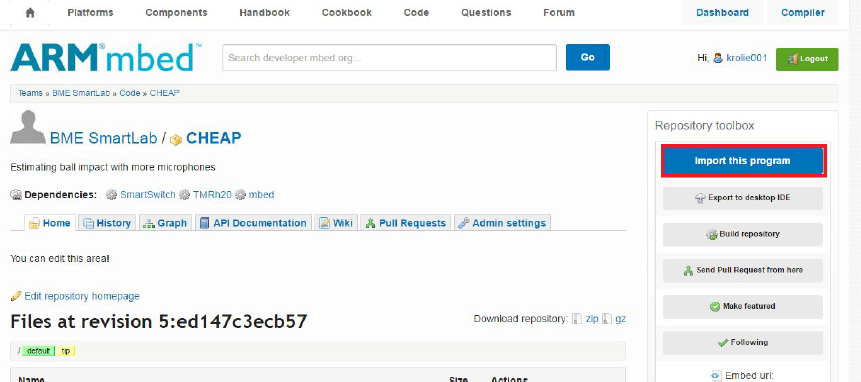
\includegraphics[width=0.9\textwidth]{figures/mbed-online-import2.png}
\end{figure}


\section{Attaching sensors and actuators}

Sensors are available as standalone modules (or simple components). After they are attached to the controller the sensed data is sent to the micro-controller. The transmission of the data can vary. Simple sensors provide analogue signals that is digitalized by the micro-controller's A/D converter. More complex sensors digitalize analogue signals and transmit digital data towards the micro-controller. These devices provide configuration capabilities on top of reading out data. The communication with these sensors are mainly consists of transmitting command words that is executed by the sensor and returns the results of the operation for the micro-controller. Complex sensors are capable of managing other sensors and return aggregated data for the micro-controller (sensor fusion). The physical communication standard between a sensor and the micro-controller is usually one of SPI, I2C, USART, OneWire, CAN, etc.

The sensors used in this lab can be retrieved from the lab demonstrator. A wide variety of sensors are available ranging from very simple to more complex ones. A complex sensor does not necessary implies complex attachment procedure. If one can't find a readily available code for connecting a given sensor it can be written during the class.

\section{Connecting a communication module}

\subsection{Nucleo board pinout}

The Nucleo F446RE board's pinout is shown of Figure~\ref{fig:nucleo-pinout}.

\begin{figure}[H]
    \centering
    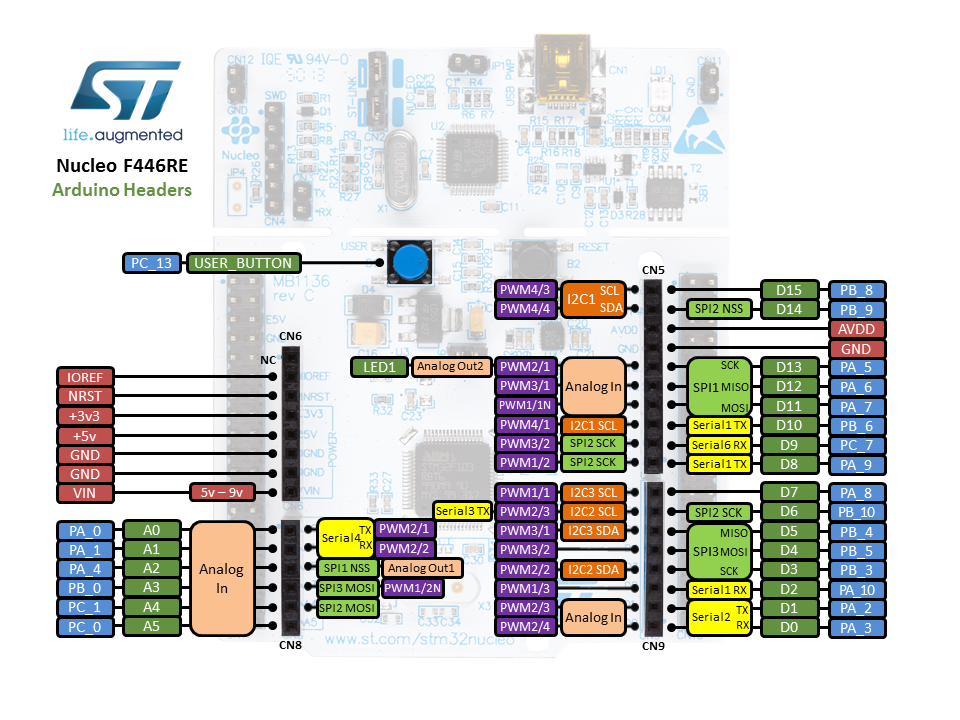
\includegraphics[width=0.9\textwidth]{figures/nucleo-pinout.png}
    \caption{Nucleo F446RE pinout}
    \label{fig:nucleo-pinout}
\end{figure}

The pins labeled are the female connectors that can be easily addressed from the mbed development environment.
Furthermore all of the 64 male connectors of the Nucleo board is accessible. The male connector header is found right beside the female connector header the only twist is that in the right side female header there is a half pin pause due to providing Arduino compatibility. The neighboring male header does not have this pause that means for a given female connector it's corresponding male connector is located in the bottom right position.
Figure~\ref{fig:nucleo-pinout-morpho} illustrates the male connector pinout.

\begin{figure}[H]
    \centering
    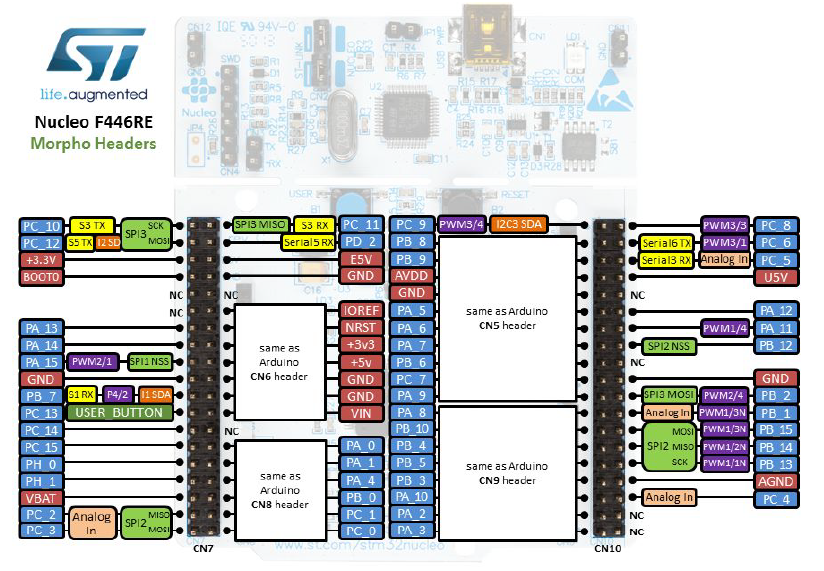
\includegraphics[width=0.9\textwidth]{figures/nucleo-morpho-pinout.png}
    \caption{Nucleo F446RE morpho pinout}
    \label{fig:nucleo-pinout-morpho}
\end{figure}

When supplying power for external devices extreme caution must be taken about the components that require 3.3V power supply \textbf{MUST NOT} be connected to a 5V supply. (e.g. the radio module requires 3.3V supply).
3.3V power supply is available in three locations: on the Arduino headers there is one male and one female connector and also on the outer header the 3rd pin from the top on the left side (according to the image).

\subsection{NRF24L01+ module pinout}

The NRF24L01+ radio module is a device communicating on SPI bus. It's important that the power supply must not exceed 3.3V!
In case of improper connection the device will be damaged permanently.
This module has power supply pins (GND,VCC) and SPI bus pins (MISO,MOSI,SCK) and 2 SPI bus control pins (CE,CSN). Furthermore there is an interrupt pin (IRQ) that is not used in these exercises so that it can be left not connected.
The pinout of the NRF24L01+ module's pinout is show of Figure~\ref{fig:radio-pinout}

\begin{figure}[H]
    \centering
    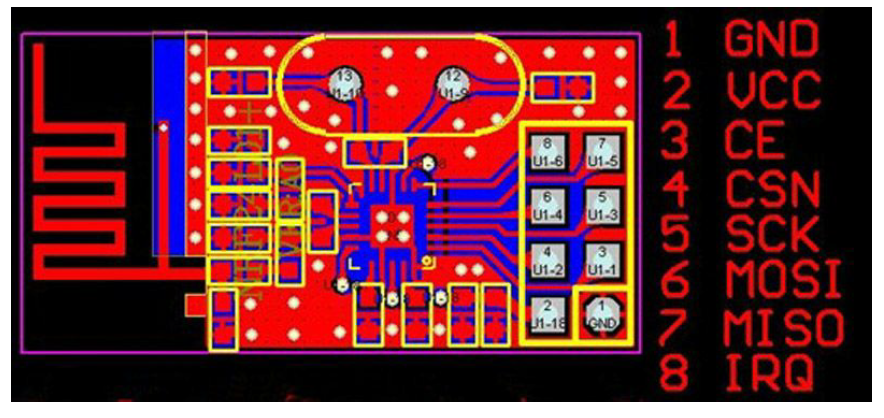
\includegraphics[width=0.9\textwidth]{figures/radio-pinout.png}
    \caption{NRF24L01+ pinout}
    \label{fig:radio-pinout}
\end{figure}

\subsection{Connecting Nucleo and NRF24L01+ modules}

Based on the pinout diagrams connecting the two devices is trivial. There is only one complication about CE and CSN pins because they can be placed freely. It is advised that D9 and D10 pins are used for this purpose because in that case they will be collocated with the SPI pins. It must not be forgotten that the radio software has to be adjusted according to the actual pinout used (NodeConfig class). An example of the interconnection is shown of Figure~\ref{fig:radio-nucleo-connection}
A sample program for the radio module connection can be downloaded from \url{https://www.tmit.bme.hu/sites/default/files/attachments/nRF24Test_TMRh20_zip_nucleo_f446re.zip}.

\begin{figure}[H]
    \centering
    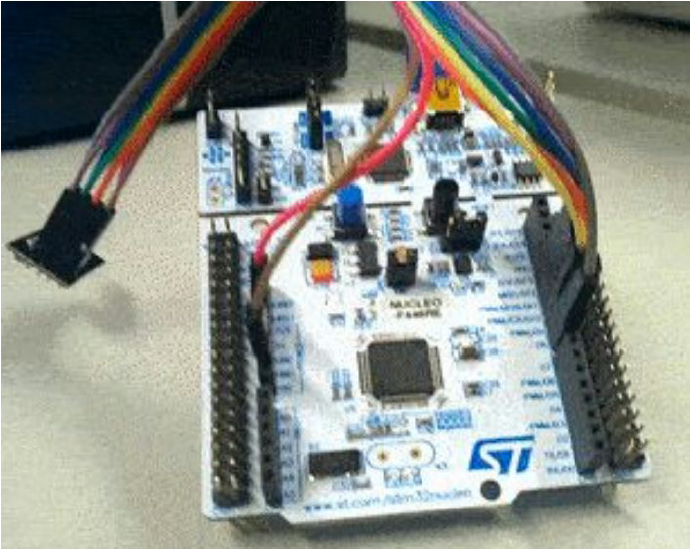
\includegraphics[width=0.9\textwidth]{figures/board-radio-example.png}
    \caption{An example of interconnecting Nucleo F446RE and NRF24L01+}
    \label{fig:radio-nucleo-connection}
\end{figure}

\section{ Virtuális eszköz készítése}

Több szolgáltató is ajánl tárhelyet IoT alkalmazásokhoz. A szolgáltatóknál tárolni és akár elemezni is lehet az adatokat. Az adatok feltöltése az Interneten keresztül történik. Ehhez a szolgáltatók API-t kínálnak. A legnépszerűbb feltöltési és hozzáférési forma a HTTP protokollt használja, de találunk olyan helyet is, ahol az MQTT protokollt használhatjuk. A méréshez egy ilyen helyet használunk az MQTT protokollal együtt. Az MQTT protokoll egy publish/subscribe protokoll, az adatokat el kell küldeni a megfelelő csatornán (topic), illetve ahhoz, hogy adathoz jussunk fel kell iratkozni a megfelelő csatornára.

IDE kell :IoT1 - DeviceHub.pdf

\section{Átjáró beállítása es MQTT kommunikáció}
 
A szenzor és a beavatkozó a saját hálózatában szállítja az adatokat, az Internet továbbításhoz szükséges az átjáró is. Az átjáró lesz, ami a szenzorhálózatos adatokat a megfelelő MQTT csatornára helyezi. Sokszor nem csak a megfelelő csatornába helyezés a feladat, hanem az adatok formátumát is igazítani kell a tároló/feldolgozó bemenetéhez. A mostani mérésnél a szenzorhálózat adatai nyers formátumban vannak, azért, hogy minél tömörebb legyen ábrázolásuk. A felhasznált felhő szolgáltató viszont JSON formátumban várja és küldi az adatot. Az átjárót fel kell konfigurálni, hogy az átalakítást elvégezze.

Példa kód:

%https://developer.mbed.org/teams/BME-SmartLab/code/DeviceHubNet_DEMO/

IDE kell :DeviceHub.net - NRF átjáró konfiguálása.pdf

\appendix

\section{Entry quiz sample questions}

\begin{enumerate}
    \item Describe briefly the main concept of the OpenFlow recommendation.
    \item What are the components of an OpenFlow network?
\end{enumerate}

\section{Lab exercises}

1.0 Hello World
Mérési feladat

    Jelentkezzen be az mbed oldalára. Válassza ki a platformok közül a NUCLEO-F446RE-t.
    Készítsen programot, amely a fejlesztői lapon található ledet villogtatja.
    Használja az mbed által nyújtott példaprogramokat!
    Készítsen programot, amely a lapon található gomb segítségével vezérli a ledet.
    Készítsen programot, amely képes a méréshez kapcsolt PC-vel kommunikálni. A kommunikációhoz soros terminált használjon. (A "minicom" ajánlott)

2.1 Szenzor és beavatkozó illesztése
Mérési feladat

    Válasszon egyet a rendelkezésre álló szenzorok és beavatkozók közül és készítsen/keressen hozzá kódot, amellyel a szenzor értékeit megjelenítheti a PC-n.
    Keresse meg a szenzorhoz tartozó adatlapot és tanulmányozza! Az illesztés során ügyeljen az adatlapon leírtak betartására!
    Illessze a szenzort a laphoz közvetlenül vagy breadboard segítségével. Amennyiben szükséges használjon egyéb alkatrészeket.
    Készítsen programot, amely a szenzor adatait szabályos időközönként megjeleníti tömör formátumban.

2.2 Kommunikáció illesztése
Mérési feladat

    Illessze a rádiós egységet a laphoz. Az rádió SPI felületen csatlakozik. Azonosítsa a megfelelő lábakat és kösse össze azokat. Ügyeljen, hogy a szenzor és a rádió ne zavarja egymás kommunikációját.
    A rádió illesztéséhez szükséges programkönyvtárakat töltse le az mbed gyűjteményéből, illetve kérje el a mérésvezetőtől.
    Ismerje meg a kommunikációs modul használatát a mérésvezetőtől kapott példaprogramon keresztül.
    Ellenőrizze a kommunikációt az átjárónál. Próbálja ki, hogy oda-vissza működik a kommunikáció.

2.3 Szenzor és beavatkozó életrekeltése
Mérési feladat

    Egyesítse a szenzor és a kommunikáció kódját. A szenzor által mért jeleket küldje el az átjárónak.
    A meglévő kódhoz adja hozzá a beavatkozó kódját.

3.1 Virtuális eszköz készítése
Mérési feladat

    Jelentkezzen be a devicehub.net oldalára és végignavigálva ez egyes menüpontokon készítse el első projektjét, a projekthez tartozó első virtuális eszközét, majd az ahhoz tartozó szenzort és beavatkozót.
    Jegyezze fel a szenzor és a beavatkozó eléréséhez szükséges paramétereket.
    Vizsgálja meg miként érhetőek el a szenzor és beavatkozó adatok az MQTT protokollon keresztül.

3.2 MQTT kommunikáció
Mérési feladat

    Tanulmányozza át az MQTT protokollt. Vizsgálja meg a megoldás egyes elemeit.
    Egy MQTT kapcsolódásra képes eszközzel létesítsen kapcsolatot egy MQTT brokerrel, majd küldjön és fogadjon üzeneteket a program segítségével. A mérőgépen az MQTTfx nevű alkalmazás van telepítve. Használhat más alkalmazást is.
    Küldjön üzeneteket a virtuális eszközének és fogadjon onnan üzeneteket. Az üzenetek formátumát és a csatornákat az előző pontban megvizsgált leírásban találja.

4.1 Átjáró beállítása
Mérési feladat

    Kérje el a mérésvezetőtől az átjáró eléréséhez szükséges paramétereket (Az átjáró elérése mérésenként változhat)
    A megtalálható példák segítségével konfigurálja az átjárót, hogy a megfelelő formátumra alakítást végezze, illetve a megfelelő csatornát válassza.
    Küldjön valós szenzoradatokat a virtuális eszköznek és a valós aktuátor fogadjon virtuális adatokat.

\subsection{Lab environment}

\end{document}